\documentclass[14pt]{extarticle}

\begin{document}
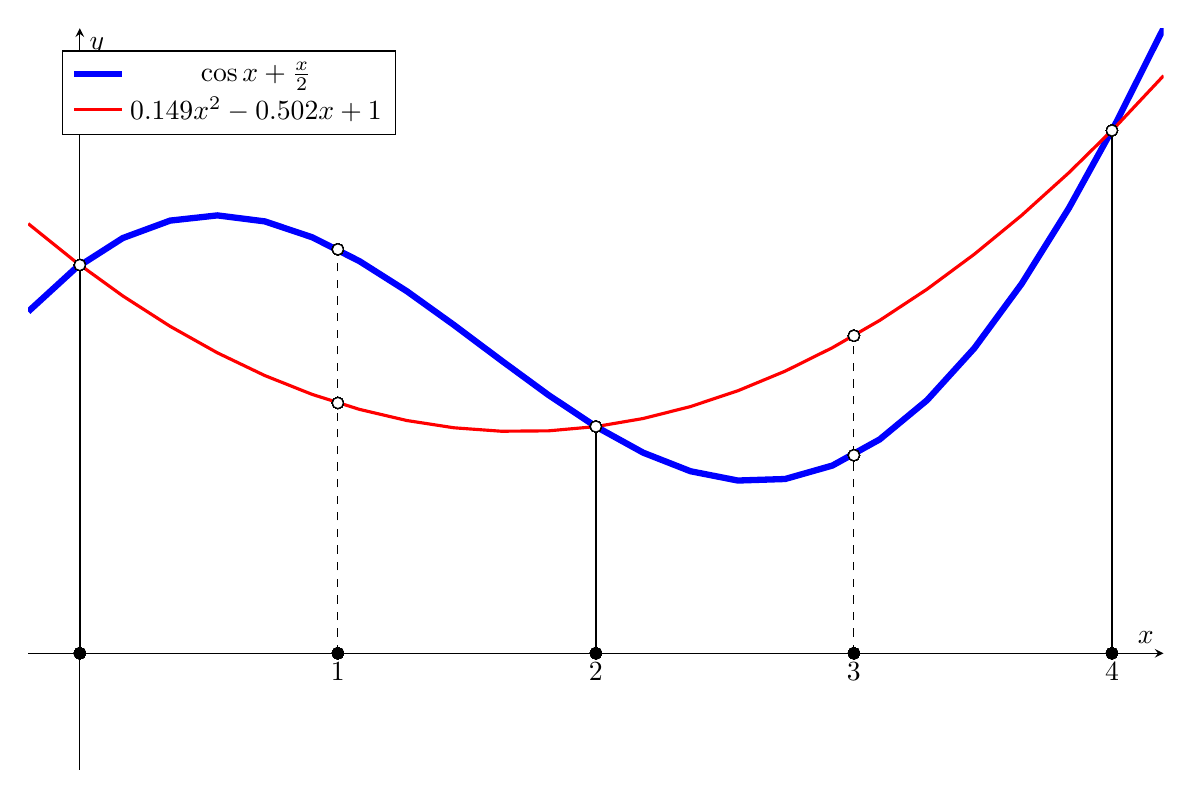
\begin{tikzpicture} [
	declare function= {
		u(\x) = cos(\x / pi * 180) + \x/2;
		subpolynonominal(\x,\A,\b,\c) = (\x-\b)*(\x-\c) /
			((\A-\b)*(\A-\c)) * u(\A);
		lag(\x,\a,\b,\c) =
			subpolynonominal(\x,\a,\b,\c) +
			subpolynonominal(\x,\b,\c,\a) +
			subpolynonominal(\x,\c,\a,\b);
	},]
	\begin{axis} [
		height=11cm,
		width=16cm,
		xlabel = {$x$},
		ylabel = {$y$},
		axis x line = middle,
		axis y line = middle,
		ymin = -0.3,
		domain = -0.2:4.2,
		ticks = none,
		legend pos = north west ]

		\newcommand*{\varA}{0}
		\newcommand*{\varB}{2}
		\newcommand*{\varC}{4}
		\newcommand*{\queryA}{1}
		\newcommand*{\queryB}{3}
		\pgfmathsetmacro{\fa}{u(\varA)}
		\pgfmathsetmacro{\fb}{u(\varB)}
		\pgfmathsetmacro{\fc}{u(\varC)}
		\pgfmathsetmacro{\Rfirst}{lag(\queryA,\varA,\varB,\varC)}
		\pgfmathsetmacro{\Rsecond}{lag(\queryB,\varA,\varB,\varC)}
		\pgfmathsetmacro{\RfirstTrue}{u(\queryA)}
		\pgfmathsetmacro{\RsecondTrue}{u(\queryB)}

		\addplot[color=blue, line width=.08cm]{u(x)};
		\addplot[color=red, line width=.04cm]{lag(x,\varA,\varB,\varC)};

		\coordinate(A) at 	(\varA,		\fa);
		\coordinate(Ap) at	(\varA,		0);
		\coordinate(B) at 	(\varB,		\fb);
		\node[below](Bp) at	(\varB,		0) {$\varB$};
		\coordinate(C) at 	(\varC,		\fc);
		\node[below](Cp) at	(\varC,		0) {$\varC$};
		\coordinate(Q1) at 	(\queryA,	\Rfirst);
		\node[below](Q1p) at	(\queryA,	0) {$\queryA$};
		\coordinate(Q1true) at	(\queryA,	\RfirstTrue);
		\coordinate(Q2) at 	(\queryB,	\Rsecond);
		\node[below](Q2p) at	(\queryB,	0) {$\queryB$};
		\coordinate(Q2true) at	(\queryB,	\RsecondTrue);

		\addplot[mark=*,only marks, fill=white]
			(\varA,\fa) node[above, pos=1]{};
		\addplot[mark=*,only marks, fill=white]
			(\varB,\fb) node[above, pos=1]{};
		\addplot[mark=*,only marks, fill=white]
			(\varC,\fc) node[above, pos=1]{};
		\addplot[mark=*,only marks, fill=white]
			(\queryA,\Rfirst) node[above, pos=1]{};
		\addplot[mark=*,only marks, fill=white]
			(\queryA,\RfirstTrue) node[above, pos=1]{};
		\addplot[mark=*,only marks, fill=white]
			(\queryB,\Rsecond) node[above, pos=1]{};
		\addplot[mark=*,only marks, fill=white]
			(\queryB,\RsecondTrue) node[above, pos=1]{};
		\addplot[mark=*,only marks, fill=black]
			(\varA,0) node[above, pos=1]{};
		\addplot[mark=*,only marks, fill=black]
			(\varB,0) node[above, pos=1]{};
		\addplot[mark=*,only marks, fill=black]
			(\varC,0) node[above, pos=1]{};
		\addplot[mark=*,only marks, fill=black]
			(\queryA,0) node[above, pos=1]{};
		\addplot[mark=*,only marks, fill=black]
			(\queryB,0) node[above, pos=1]{};

		\draw[thick] (Ap) -- (A)  (Bp) -- (B)  (Cp) -- (C);
		\draw[dashed] (Q1p) -- (Q1true)	(Q2p) -- (Q2);

		\addlegendentry{$\cos x+\frac{x}{2}$};
		\addlegendentry{$0.149x^2-0.502x+1$};
	\end{axis}
\end{tikzpicture}
\end{document}
